%!TEX root = /Users/andy/Documents/Academics/Dissertation/thesis.tex




multiplexed snp genotyping site:ncbi.nlm.nih.gov

\chapter{Sub-micrometer Geometrically Encoded Fluorescent Barcodes Self-Assembled from DNA}

\section{Introduction}
%Comment to chenxiang: found the beginning cheesy,modified it a bit
\newthought{In biology and medicine} researchers often use fluorescence microscopy to visualize nanometer to micrometer-sized entities. In many cases it is desirable to visualize more than one class of objects simultaneously and unambiguously. As such there is a need to develop suitable 
fluorescent tags (barcodes) for multiplexed imaging applications. Most previously 
described fluorescent barcodes are constructed using either intensity encoding \citep{han_quantum-dot-tagged_2001,xu_multiplexed_2003,li_multiplexed_2005,livet_transgenic_2007,fournier-bidoz_facile_2008,lin_self-assembled_2007,marcon_--fly_2010} or 
geometrical encoding \citep{nicewarner-pena_submicrometer_2001,gudiksen_growth_2002,braeckmans_encoding_2003,dejneka_rare_2003,geiss_direct_2008,pregibon_multifunctional_2007,xiao_direct_2009,li_controlled_2010}. Intensity encoding relies on the combination of multiple 
spectrally differentiable fluorophores in a controlled molar ratio. Geometrical encoding, 
on the other hand, is obtained by separating optical features beyond the microscope’s 
resolution limit (typically \textasciitilde250 nm for diffraction-limited imaging and \textasciitilde 50 nm for 
current super-resolution imaging) and arranging them in a specific geometric pattern.
%ANDY ADDED the following
Here we combine both intensity and geometric methods. The multiplexing capability of geometrically encoded barcodes increases 
exponentially as additional spatially distinguishable fluorophores are incorporated. 
Therefore, larger barcode libraries may be more easily accessible through geometrical 
encoding, provided that a rigid structural scaffold capable of defining the spatial 
arrangement of the fluorescent molecules is available. To date, despite the remarkable 
success in synthesizing fluorescent barcodes for in vitro multiplexed detection, very little 
effort has been made to create robust single-molecule barcodes suitable as in situ imaging 
probes. In addition, most existing fluorescent barcodes range from 2 \textmu m to 100 \textmu m in 
size, leaving the construction of fluorescent barcodes with largest dimension less than 1 
\textmu m an underexplored research area (with only a few reports  \citep{li_multiplexed_2005,lin_self-assembled_2007,li_controlled_2010,levsky_single-cell_2002} and no more than 11 
distinct barcodes experimentally demonstrated). Here we report a group of geometrically and intensity 
encoded fluorescent barcodes self-assembled from DNA that can be used to tag yeast 
cells. These barcodes are 400–800 nm in length, structurally rigid, biocompatible, 
reprogrammable in a modular fashion and easy to decode using epi-fluorescence, total internal reflection fluorescence (TIRF) or 
super-resolution fluorescence microscopy. As evidence of the multiplexing power of the 
system, 216 distinct barcode species (20 times more than previously experimentally 
demonstrated systems) were constructed and resolved using diffraction-limited TIRF 
microscopy. 

%Comment for Chenxiang: Way Way Way too many references. Many of these are wholly irrelevant! 
Structural DNA nanotechnology takes advantage of the well-defined double 
helical structure of DNA and the highly predictable Watson-Crick base-paring rules to 
self-assemble designer nano-objects and devices \citep{seeman_nucleic_1982,aldaye_assembling_2008,lin_designer_2009,nangreave_dna_2010,shih_knitting_2010,trring_dna_2011}. In recent years, DNA origami has 
emerged as a prominent method to fabricate two- and three-dimensional structures with 
sizes of tens to hundreds of nanometers \citep{rothemund_folding_2006,douglas_self-assembly_2009,dietz_folding_2009,ke_multilayer_2009,andersen_self-assembly_2009,han_folding_2010,liedl_self-assembly_2010,han_dna_2011}. By folding a long, single-stranded DNA 
molecule (a scaffold strand, often times an M13 viral genomic DNA or its derivatives) 
with the help of many short synthetic DNA oligonucleotides (staple strands), this 
approach generates complex, shape-controlled, fully addressable nanostructures. With 
certain functional groups attached to selected staple strands or their extensions, such 
nanostructures can be used to organize fluorescent guest molecules, including small 
organic molecules \citep{jungmann_single-molecule_2010,steinhauer_dna_2009,lund_molecular_2010} as well as metallic \citep{pal_dna-origami-directed_2010} and semi-conductive nano-particles \citep{bui_programmable_2010}. In 
addition, individual DNA-origami nanostructures can be joined together in a 
programmable way to make micrometer-sized structures while maintaining their unique 
nanometer scale spatial addressability \citep{liu_crystalline_2011,woo_programmable_2011}. These properties make DNA origami 
promising material to build robust fluorescent barcodes, as control over the exact ratio of 
different fluorophores allows intensity encoding while spatial positioning of fluorophores 
facilitates geometrical encoding and can help minimize undesired inter-fluorophore 
quenching. 

\section{DNA Origami Barcode Construction}
\subsection{A Simple Barcode}
As a proof-of-concept demonstration, we first designed a family of 27 barcodes 
based on six-helix bundle DNA nanotubes \citep{douglas_dna-nanotube-induced_2007} that are ~800 nm long. Figure \ref{fig:dna1}a illustrates 
the design of such barcodes. Three 84-base pair (\textasciitilde28 nm) zones on the nanotube were 
selected for fluorescent labeling, with inter-zone distances of 450 nm and 270 nm 
between the first and the last two zones, respectively. In this design, the fluorescently 
labeled zones were separated beyond the diffraction limit of visible light (\textasciitilde250 nm) and 
the symmetry of the nanotube was broken so that the barcodes could be geometrically 
encoded with a distinguishable “head” and “tail”. For example, labeling the three zones 
(from left to right in Figure \ref{fig:dna1}a) with “Blue” (B, Alexa Fluor 488), “Red” (R, Alexa Fluor 
647) and “Green” (G, Cy3) fluorophores (the pseudo-colors were assigned to reflect the 
excitation wavelength of the fluorophores) resulted in a BRG barcode that should be 
distinguishable from a GRB barcode. Therefore, a total of $3^{3}=27$ different barcodes can 
be made from three spectrally distinguishable fluorophores. Within each zone (Figure 
\ref{fig:dna1}b), fluorescently modified oligonucleotides were hybridized to the twelve 21-base long 
staple extensions protruding out from the main body of the nanotube. The distance 
between adjacent staple extensions was \textasciitilde6 nm. In order to image these prototype 
barcodes in our prototype experiments, ten additional staple strands (five per monomer) 
were designed with 5' biotinylated extensions to enable surface attachment (See Figure 
\ref{fig:dnaS1} for the full design blueprint as strand diagram). 


\begin{figure} %1 
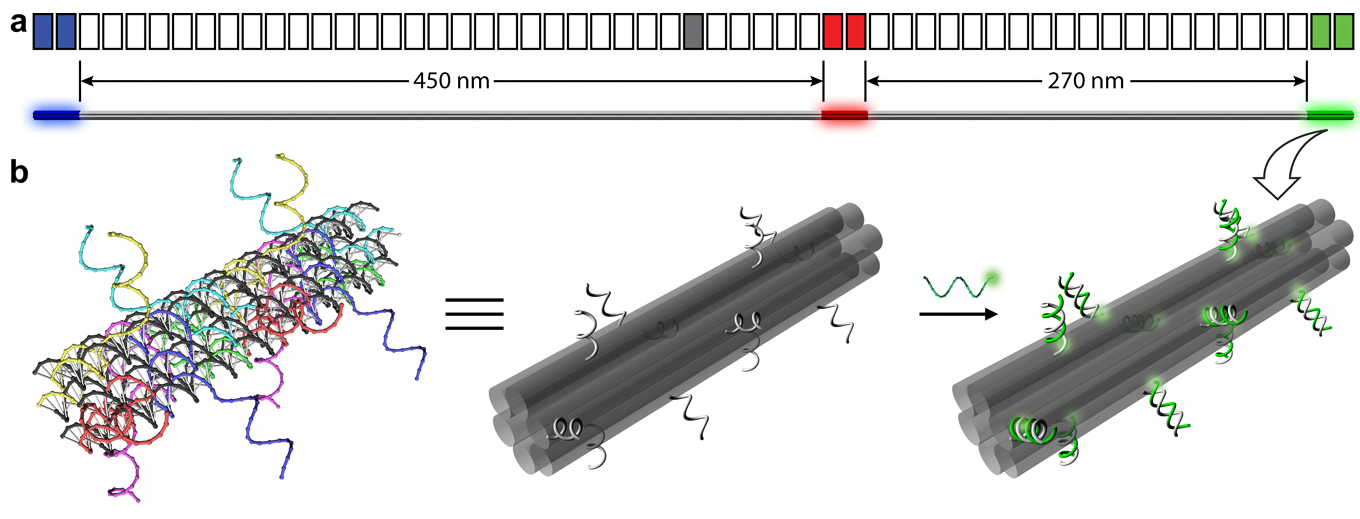
\includegraphics[width=\textwidth]{figures/dna1}
\caption[Design of the DNA-nanotube-based barcode.]{ Design of the DNA-nanotube-based barcode. (\textbf{a}) Two schematic drawings of 
the Blue--Red-Green (BRG, “--” and “-” denotes larger and smaller inter-zone distance in 
the barcode, respectively) barcode with a segment diagram on the top and a 3D view at 
the bottom. The main-body of the barcode is a DNA nanotube formed  by  
dimerizing two origami monomers, each consisting of 28 segments of length 42-bp (13.6 nm).
The grey segment in the middle represents the junction where the two monomers 
are joined together through cross-hybridization between their scaffolds and staples. Three 
84-bp zones of the nanotube are fluorescently labeled (shown as blue, red and green 
segments) to produce the BRG barcode with an inter-zone distance of 450 nm between 
the first two zones and 270 nm between the last two. Note that each zone is only labeled 
with one fluorophore species. The resulting barcodes are thus referred as single-labeled- 
zone barcodes. (\textbf{b}) 3D cartoons showing the details of one fluorescently labeled zone. 
Left: a scaffold-plus-staple model of such an 84-bp zone before labeling. Each of the 
twelve 63-base-long staples (shown in rainbow colors) contains two parts: the 42-base 
region at the 5'-end weaves through three double-helices to fold the scaffold (shown in 
black) into a six-helix bundle nanotube; and the 21-base extension at the 3'-end protrudes 
out for fluorescent labeling. Middle: an identical but simplified model to emphasize the 
six-helix bundle structure (each helix shown as a semi-transparent grey cylinder) and the 
positioning of the twelve 21-base staple extensions (each shown as a light-grey curl). 
Right: Cartoon representation of a “green” 84-bp zone. The labeling is achieved by 
hybridizing the Cy3 (shown the glowing green spheres at the 3'-ends) modified strands to 
the staple extensions.\label{fig:dna1}}
\end{figure}


We assembled the DNA-origami nanotubes following the protocol in \citep{douglas_dna-nanotube-induced_2007} with slight experimental modifications (See Materials and Methods in SI). 
Briefly, two structurally identical but chemically distinct nanotube monomers (\textasciitilde400 nm 
each) were assembled in two separate test tubes by slowly cooling a mixture of 7.3-kb 
scaffold strands and a set of \textasciitilde200 staple strands from 80 \textdegree C to 24 \textdegree C over 15 hours. After 
folding, excessive staple strands were removed from the folded nanotubes through 
polyethylene glycol fractionation. The nanotube monomers were then incubated with the 
desired fluorescently modified oligonucleotides and the labeled monomers were mixed at 
an equimolar ratio to form the final barcode structure. The barcodes were subsequently 
purified via agarose-gel electrophoresis and immobilized on streptavidin-coated 
coverslips before imaging with epi-fluorescence (Figure \ref{fig:dna_s2}) or TIRF microscopy (Figure 
\ref{fig:dna2} and \ref{fig:dna3}) in the presence of oxygen scavenging reagents \citep{liedl_self-assembly_2010}. 

\begin{figure} %2
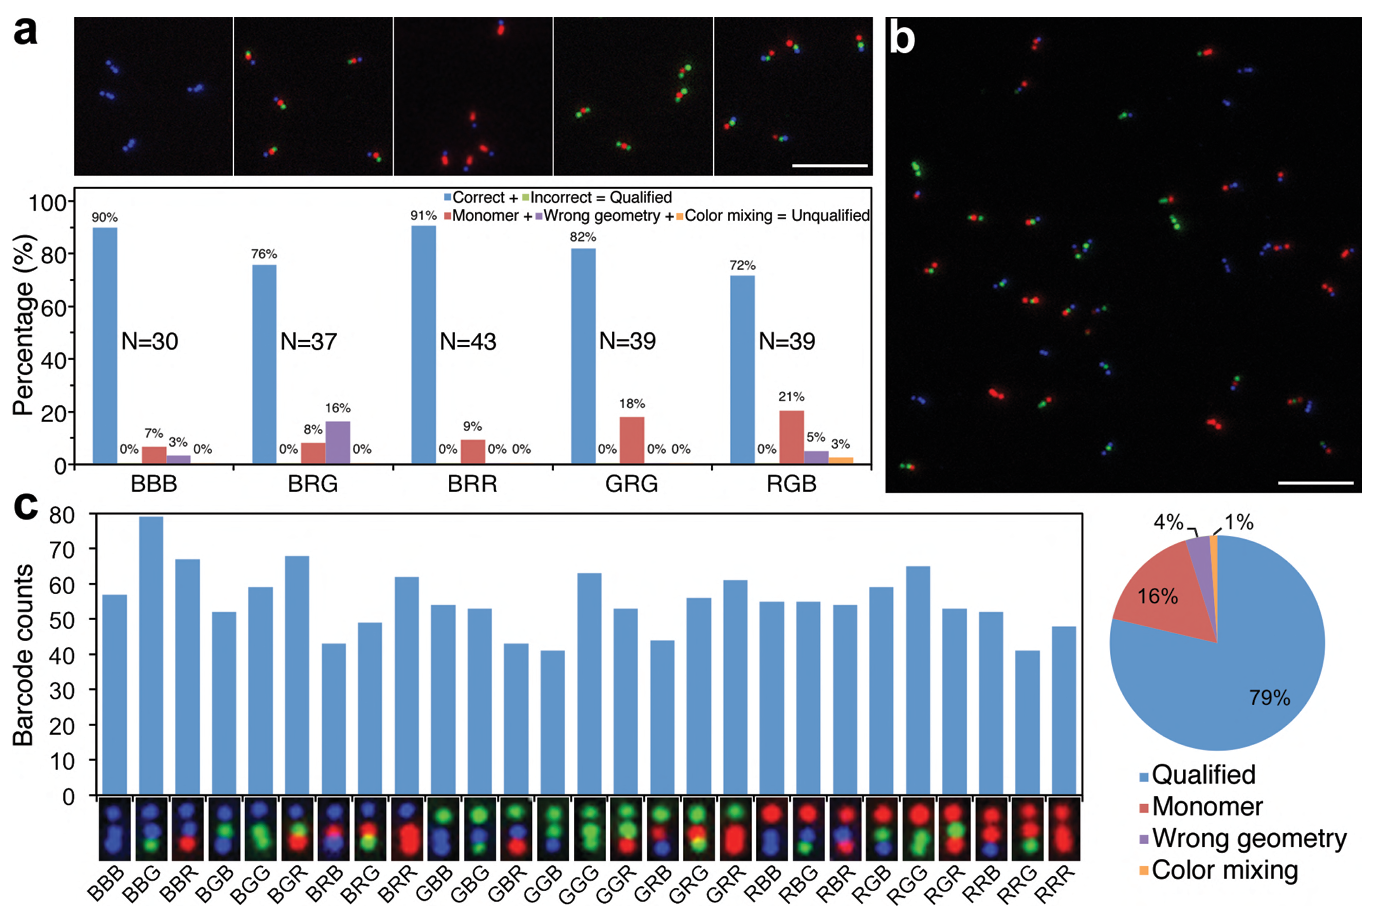
\includegraphics[width=\textwidth]{figures/dna2}
\caption[Single-labeled-zone fluorescent barcodes.]{Single-labeled-zone fluorescent barcodes. (\textbf{a}) Superimposed TIRF microscopy 
images of five barcode species (top) and the statistics from manual counting (bottom). 
From left to right are the BBB, BRG, BRR, GRG and RGB barcodes with a 
representative image on top of the corresponding bar-graph. Each bar-graph is generated 
based on the manual sorting and counting of the objects found in a 50×50 \textmu m$^2$ image 
(\textasciitilde40 barcodes, the exact sample size N is noted beside the corresponding bar-graph). (\textbf{b}) 
A representative image of the equimolar mixture of 27 barcode species. (\textbf{c}) Statistics 
obtained by analyzing twenty-seven 50×50 \textmu m$^2$ images of the 27 barcode mixture 
(\textasciitilde1,500 barcodes in total). Left: barcode counts of the 27 species (average count of 55 
with a standard deviation of 9). A representative TIRF image (1.4×0.7 \textmu m$^2$) of each 
barcode type is placed underneath the corresponding bar. Right: sorting result of the 
observed objects shown as a pie-chart. Color scheme used for the bar-graphs and the pie- 
chart (unrelated to the pseudo-colors of the fluorophores): blue, correct barcodes 
(qualified barcode with expected identity); green, incorrect barcodes (qualified barcode 
with unexpected identity); red, monomer nanotubes (one spot or two connecting spots); 
purple, barcodes with wrong geometry (i.e., bending angle <120\textdegree, see methods in SI); 
and orange, barcodes containing at least one spot with two colors. Note that in the 27- 
barcode pool, correct vs. incorrect barcodes were not distinguishable because all barcode 
types are expected. As a result the bars and pie representing the qualified barcodes in (\textbf{c}) 
are shown in blue. Scale bars: 5 \textmu m.\label{fig:dna2}}
\end{figure}
	



%Andy, don't forget to go back and add references to Supplementary Information and Supplementary Figures



\section{Manuscript Information}
\subsection{Submitted for Publication As}
A version of this chapter has been submitted for publication in the journal \textit{Nature Nanotechnologies}.
% in \citep{leifer_optogenetic_2011}:
%\bibentry{leifer_optogenetic_2011}

\subsection{The Author's Contribution}
Andrew M.~Leifer conceived of and wrote the software to analyze TIRF images and identify and decode the barcodes. He wrote portions of the manuscript and generated one of the supplementary figures. 